\chapter{Théorie des graphes}
\label{partie:graph}
Cette partie s'inspire des documents \cite{koung_cooperative_2022,ren_distributed_2008,noauthor_graph_2025}.

\section{Introduction }
\label{graphes:intro}
\begin{wrapfigure}{r}{0.4\textwidth}
\vspace{-0.4cm}

  \centering
  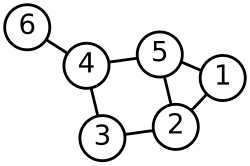
\includegraphics[width=0.38\textwidth]{Annexes/Graph_Theory/pic/graphe_example.png}
  \caption{Exemple de graphe}
  \label{fig:graph_example}
\end{wrapfigure}
La théorie des graphes est un domaine des mathématiques et de l'informatique qui s'intéresse à l'étude des graphes, des structures composées de nœuds (ou sommets) pouvant être connectés entre eux par des arêtes. Ces graphes permettent de modéliser des relations ou des interactions entre objets. Un exemple de graphe est illustré en figure \ref{fig:graph_example}. Dans le cadre des essaims de robots, cette représentation est couramment utilisée : chaque robot est associé à un nœud, et une arête peut symboliser une interaction ou une proximité, par exemple avec un robot voisin. Ainsi, la théorie des graphe permet de représenter la topologie du système.


\section{Définition mathématique }

\subsection{Principe}
Comme expliqué précédemment en introduction, un graphe $\mathcal{G}$ est composé d’un ensemble de nœuds, noté $\mathcal{E}$, et d’un ensemble d’arêtes, noté $\mathcal{V}$.
\begin{itemize}
    \item $\mathcal{V}=\{1, 2, \ldots, n\}$, l'ensemble des noeuds.
    \item $\mathcal{E}\subseteq \{(i, j) : i, j \in \mathcal{V},\ j \ne i\}$. Une arête est composée de noeuds $i$ et $j$
\end{itemize}

Un graphe peut être représenté sous la forme d'une matrice d'adjacence $\mathcal{A}(\mathcal{G})$ de taille $n \times n$ (où $n$ est le nombre de nœuds), dont les termes $a_{i,j}$ indiquent la présence ou non d’une arête entre les nœuds $i$ et $j$. Chaque élément $a_{i,j}$ de la matrice est défini par :

\[
a_{i,j} =
\begin{cases}
1 & \text{ si } (i,j) \in  \mathcal{E} \text{ c'est-à-dire une qu'il existe une arête entre les nœuds } i \text{ et } j  
 \\
0 & \text{sinon.}
\end{cases}
\]
Par exemple, sur la Figure \ref{fig:graph_example}, il y a 6 nœuds formant les arêtes suivantes :
\begin{itemize}
    \item le nœud 1 est lié au nœud 2 et au nœud 5
    \item le nœud 2 est lié au nœud 3 et au nœud 5
    \item le nœud 3 est lié au nœud 4
    \item le nœud 4 est lié au nœud 5 et au nœud 6
\end{itemize}
Il est alors possible d'en déduire la matrice d'adjacence suivante :
\[
\mathcal{A}(\mathcal{G}) =
\begin{bmatrix}
0 & 1 & 0 & 0 & 1 & 0 \\
1 & 0 & 1 & 0 & 1 & 0 \\
0 & 1 & 0 & 1 & 0 & 0 \\
0 & 0 & 1 & 0 & 1 & 1 \\
1 & 1 & 0 & 1 & 0 & 0 \\
0 & 0 & 0 & 1 & 0 & 0
\end{bmatrix}
\]

La matrice obtenue est symétrique, car le graphe est non orienté (voir Partie \ref{graphe:complément}) ce qui signifie que les connexions sont valables dans les deux sens, et la diagonale est nulle car il n'y a pas, dans ce cas, de connexion entre un nœud et lui-même.
\subsection{Propriétés}
\label{graphe:complément}

\subsubsection{Graphes orientés}

Les arêtes peuvent avoir une orientation; le graphe est alors dit \textbf{orienté}. Un exemple est donné ci-contre.
\begin{wrapfigure}{r}{0.4\textwidth}
\vspace{-0.4cm}

  \centering
  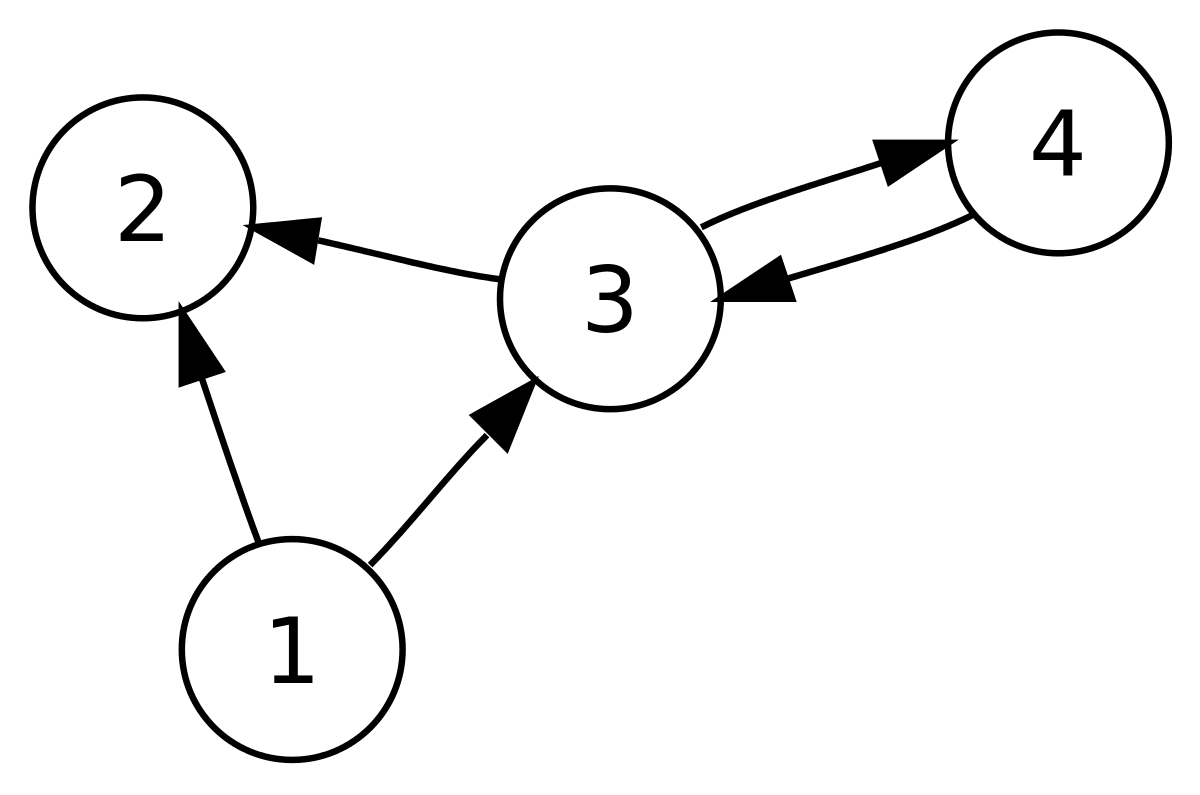
\includegraphics[width=0.38\textwidth]{Annexes/Graph_Theory/pic/oriented_graph.png}
  \caption{Graphe orienté}
  \label{fig:oriented_graphe}
\end{wrapfigure}
Dans ce cas, la matrice d'adjacence est la suivante :
\[
\mathcal{A}(\mathcal{G}) =
\begin{bmatrix}
0 & 1 & 1 & 0   \\
0 & 0 & 0 & 0   \\
0 & 1 & 0 & 1   \\
0 & 0 & 1 & 0   
\end{bmatrix}
\]
Si le graphe est orienté, la matrice d'adjacence n'est plus symétrique, sauf si toutes les arêtes sont bidirectionnelles, ce qui revient à considérer le graphe comme étant non-orienté.

\subsubsection{Connexité}

Un graphe est dit \textbf{connexe} s'il existe un chemin, pour n'importe quel couple de nœud $(i,j)$ du graphe $\mathcal{G}$ une chaîne/ un chemin reliant $i$ et $j$.

Par exemple, les graphes ci-dessous ne sont pas connexes.
\begin{figure}[h]
    \centering
    \begin{minipage}[b]{0.45\textwidth}
        \centering
        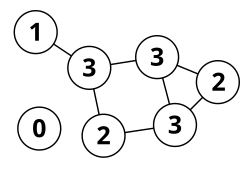
\includegraphics[width=\textwidth]{Annexes/Graph_Theory/pic/Undirectedgraphe.png}
        \caption{Exemple 1 de graphe non connexe }
        \label{fig:non connexe 1}
    \end{minipage}
    \hspace{0.05\textwidth} % Espace entre les deux images
    \begin{minipage}[b]{0.45\textwidth}
        \centering
        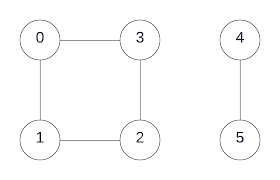
\includegraphics[width=\textwidth]{Annexes/Graph_Theory/pic/undirectedgraphe2.png}
        \caption{Exemple 2 de graphe non connexe}
        \label{fig:non connexe 2}
    \end{minipage}
\end{figure}
Sur la Figure \ref{fig:non connexe 1}, le noeud 0 n'est pas relié à d'autres nœuds, il n'existe pas de chemin reliant le nœud 0 et le nœud 1 par exemple.
Sur la Figure \ref{fig:non connexe 2}, il n'existe par exemple pas de chemin reliant le nœud 4 et le nœud 1.
Lorsqu’un graphe est orienté, plusieurs niveaux de connexité peuvent être distingués :
\begin{itemize}
\item \textbf{Connexité faible} : le graphe est connexe lorsque l’orientation des arêtes est ignorée.
\item \textbf{Connexité unilatérale} : pour chaque paire de sommets $(i,j)$, un chemin orienté existe de $i$ vers $j$ ou de $j$ vers $i$, mais pas nécessairement dans les deux sens.
\item \textbf{Connexité forte} : un chemin orienté relie chaque sommet $i$ à tout autre sommet $j$, peu importe le sens.
\end{itemize}

\subsubsection{Arbre couvrant (Spanning Tree)}
\label{graphe:spanningtree}

Un \textbf{arbre couvrant} est une sous-structure d’un graphe connexe qui relie tous les nœuds du graphe avec un minimum d’arêtes, sans former de cycle. Un graphe de $n$ nœuds possède un arbre couvrant composé de exactement $n - 1$ arêtes.
Un graphe admet un arbre couvrant \textit{si et seulement si} il est connexe.

\begin{figure}[h]
    \centering
    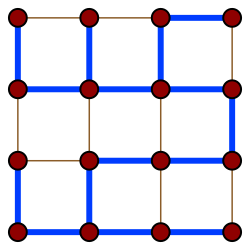
\includegraphics[width=0.4\textwidth]{Annexes/Graph_Theory/pic/4x4_grid_spanning_tree.svg.png}
    \caption{Exemple d’un arbre couvrant (en bleu)}
    \label{fig:spanning_tree}
\end{figure}

\subsubsection{Rigidité}

Un graphe est rigide si les distances (taille des arête) entre certains couples de nœuds suffisent à garantir que la structure globale de la formation ne peut pas être modifiée (par exemple être déformée ou pliée) sans altérer ces distances. En d'autres termes, la formation est préservée, à une translation ou une rotation près.

Plus formellement, un graphe est dit \textbf{rigide en dimension 2} si, pour une configuration générique des positions des nœuds dans le plan, la seule manière de déplacer les nœuds tout en conservant les longueurs des arêtes est de faire une translation ou une rotation globale de l’ensemble du graphe.

Pour qu’un graphe non orienté à $n$ nœuds soit rigide dans le plan, une condition nécessaire est qu’il possède au moins $2n - 3$ arêtes. Cependant, ce n’est pas suffisant : la répartition de ces arêtes est également importante.

Dans les applications robotiques, la rigidité garantit que les robots peuvent estimer leur position relative les uns par rapport aux autres à partir de mesures de distance locales, ce qui est essentiel pour le maintien de formations.


\section{Lien avec un essaim de robot }

Il faut choisir avec soin le type de graphe à utiliser lors de la conception d'un essaim. Dans le cadre du projet eSWARM, l'objectif est de mettre en place un système d'essaim décentralisé, ce qui implique la non orientation ainsi que la connexité du graphe. En effet, chaque agent de l'essaim doit avoir accès aux informations des autres agents de l'essaim (par exemple, les distances inter-agents ou la position du robot etc).